\section{Deep learning and Protein Contact Prediction}

    \subsection{Residual Networks (ResNets)}

        As described in section \ref{backpropagation} about backpropagation,
        the loss gradient with respect to the parameters of a specific layer
        is computed as the product of many other mathematical entities
        (vectors, scalars, matrices, etc.), and the number of factors in such
        a product grows linearly with the number of operations applied after
        current layer. When this number is too large, some layers may be
        updated with numerically unstable gradients.

        A widely used solution is to add
        \textbf{residual connections}~\cite{DBLP:journals/corr/HeZRS15}
        to the architecture. The latter can thus no longer be viewed as
        a regular composition of functions and must take into account
        the sum at the end of each residual block.
        Let's assume a residual block starts at layer $k$. Then the output
        of the residual block can still be formalized as the following:

        \begin{equation}
            Y^{(r)} = f\big(X^{(r)}, \{W^{(p)}\}_p\big)
        \end{equation}

        \todo{}

        \begin{figure}[H]
            \begin{center}
                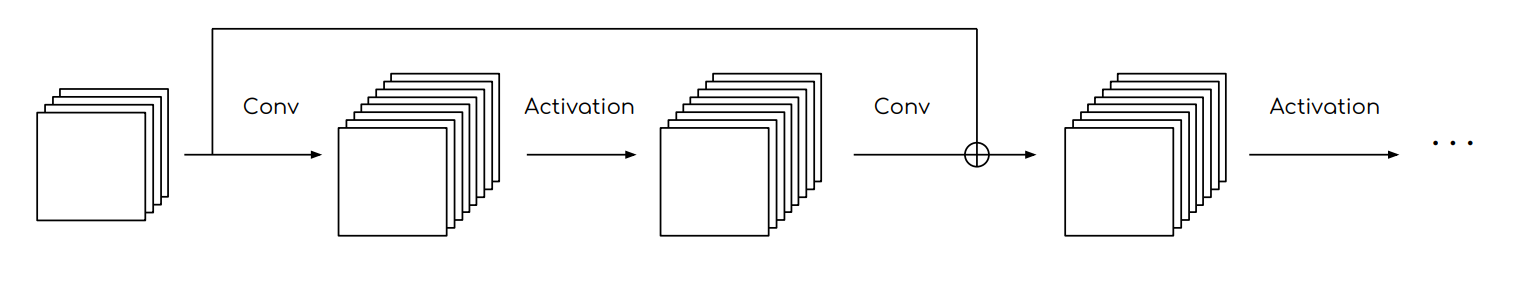
\includegraphics[width=\textwidth, keepaspectratio]{imgs/resnet.png}
                \caption{Illustration of a residual connection in a convolution
                neural network. For the element-wise sum to work, the input and output
                of the residual block are required to be of the same shape.}
                \label{resnet}
            \end{center}
        \end{figure}
    
    \todo{DNCON2: \cite{doi:10.1093/bioinformatics/bty341}}

    \todo{PConsC4: \cite{Michel383133}, zero-padding, based on U-net: \cite{DBLP:journals/corr/RonnebergerFB15}}

    \todo{DeepContact: \cite{DeepContact}}

    \todo{RaptorX-Contact: \cite{RaptorX}, zero-padding}

    \todo{DeepCov: \cite{doi:10.1093/bioinformatics/bty341}}

    \todo{TiramiProt: \cite{TsardakasRenhuldt1228846}}

    \todo{DeepConPred2: \cite{DeepConPred2}}

    \todo{plmConv: \cite{golkov2016protein}}

    \todo{proteinloopmodeling}

    Benchmark with both accuracy and standard deviation w.r.t. proteins.


    \todo{Deep architectures in PCP: \cite{di2012deep}}

    \todo{DenseNet: \cite{huang2017densely}}
